% ======================================================================
\section*{Appendix overview}
The appendix documents the implementation and analysis behind every
main-text claim.
\begin{itemize}
\item \textbf{A} the generator and its calibration (\S\ref{sec:framework},
\S\ref{sec:diverge});
\item \textbf{B} the instrumented audit of v1 confirmation scripts
(\S\ref{sec:prov}, \S\ref{sec:multitest});
\item \textbf{C} the trusted protocol (\S\ref{sec:protocols});
\item \textbf{D} fault operators and manifestation (\S\ref{sec:env});
\item \textbf{E} replay;
\item \textbf{F} statistical procedures;
\item \textbf{G} full result tables;
\item \textbf{H} reproducibility;
\item \textbf{I} construct and external validity.
\end{itemize}
Unless stated otherwise, numbers come from the frozen files under
\texttt{research\_v2/results/}, and code paths refer to the repository. The
v1 study is the original experiment (\texttt{scieval/}); v2 is the
trusted-protocol experiment (\texttt{research\_v2/}).

% ======================================================================
\section{Data-Generating Process and Statistical Calibration}
\label{app:dgp}

\subsection{Formal generative model}
\label{app:dgp-model}
A task is indexed by an integer seed $s$ and a kind
$k\in\{\text{effect},\text{null}\}$ (\texttt{scieval/tasks.py}, function
\texttt{make\_task}). A single generator
$\mathcal{R}_s=\texttt{default\_rng}(s)$ drives every random choice in the
following order:
\begin{enumerate}
\item Choose the framing $f=s\bmod 4$, with ten exposure names
$c_1,\dots,c_{10}$, an outcome name, a site name, and four site labels.
\item Draw a permutation $\pi$ of $\{1,\dots,10\}$. The decoy is
$d=\pi_1$, the text-encoded exposure is $m=\pi_2$, and in effect tasks the
true exposure is $j^*=\pi_3$.
\item In effect tasks draw $\beta\sim U(0.15,0.25)$; in null tasks
$\beta=0$ and $Z=\varnothing$.
\item Draw the exploration split, then the confirmation split, each of
$n=400$ rows, by the same row model.
\end{enumerate}
For row $r$ of a split:
\begin{align}
S_r&\sim\mathrm{Unif}\{1,2,3,4\}, \qquad \delta_{S_r}\in(-0.8,-0.3,0.3,0.8),\\
X_{rj}&\overset{iid}{\sim}N(0,1)\quad (j\neq d), \qquad X_{rd}=U_{rd}+1.2\,\delta_{S_r},\ U_{rd}\sim N(0,1),\\
Y_r^\star&=\delta_{S_r}+\beta X_{rj^*}+\varepsilon_r,\qquad \varepsilon_r\sim N(0,1).
\end{align}
Recorded columns are affine rescalings rounded to three decimals: exposure
$=\mathrm{round}(10+2X_{rj},3)$ and outcome $=\mathrm{round}(50+5Y^\star_r,3)$.
Site is stored as its text label. Then:
\begin{itemize}
\item $\lfloor n/100\rfloor=4$ randomly chosen outcomes are set missing;
\item $\lfloor 3n/100\rfloor=12$ randomly chosen entries of exposure $m$
are replaced by the string \texttt{"NA"}, so the column is stored as text.
\end{itemize}
Because the two splits are consecutive draws from $\mathcal{R}_s$, they are
independent samples from the same distribution conditional on the task
parameters $(f,\pi,\beta)$. Every quantity that matters for inference is
invariant to the affine rescaling, since $t$-statistics are scale-free.

This is a controlled statistical generating process, not a general
observational causal problem. The only confounding path is the designed one
($S\to X_d$, $S\to Y$). Exposures other than the decoy are independent of
site and of each other. All effects are positive. The correct analysis,
OLS with site indicators, is known to the designers.

\subsection{Why site adjustment matters}
\label{app:dgp-ovb}
Let $\sigma_\delta^2=\mathrm{Var}(\delta_S)=\tfrac14(0.64+0.09+0.09+0.64)=0.365$.
In a null task the decoy has no direct effect, but its marginal regression
slope on the latent scale is
\begin{equation}
\frac{\mathrm{Cov}(Y^\star,X_d)}{\mathrm{Var}(X_d)}=\frac{1.2\,\sigma_\delta^2}{1+1.44\,\sigma_\delta^2}=\frac{0.438}{1.526}=0.287,
\qquad
\rho(Y^\star,X_d)=\frac{0.438}{\sqrt{1.365\times1.526}}=0.304 .
\end{equation}
With $n\approx 396$ complete rows the unadjusted $t$-statistic is about
$\rho\sqrt{n-2}/\sqrt{1-\rho^2}\approx 6.3$, so an unadjusted test rejects
essentially always. The simulation agrees: 5,000 of 5,000 null pairs reject
(Table~\ref{tab:dgp}).

The true exposure in an effect task has marginal correlation
$\beta/\sqrt{1.365+\beta^2}\approx0.13$--$0.21$ and $t\approx 2.6$--$4.2$.
An unadjusted screen therefore prefers the decoy. Simulation gives 100\% decoy
selection on nulls and only 3.6\% correct discoveries on effect tasks when the
naive screen is followed by an adjusted test. Conditioning on site removes the
path, because $X_d\perp Y^\star\mid S$ when $\beta=0$ or $d\neq j^*$. The
site-adjusted test of the decoy then rejects at the nominal rate (4.7\%). The
locked test of the true exposure has site-adjusted standard error about
$1/\sqrt{n}$ on the latent scale, which gives $t\approx\beta\sqrt{n}\approx
3.0$--$5.0$.

\subsection{Exploration versus confirmation}
\label{app:dgp-selection}
Let $\mathcal{D}^E$ and $\mathcal{D}^C$ be the two splits. A policy picks
$\hat H=g(\mathcal{D}^E)$, any function of exploration data however many
comparisons it makes, and then tests $\hat H$ once on $\mathcal{D}^C$. Under
the null, $\mathcal{D}^C\perp\mathcal{D}^E$, so
$\Pr(p_{\hat H}(\mathcal{D}^C)<\alpha)=\alpha$. The single confirmatory test
keeps its nominal size, which the simulation reproduces (4.8\%). The
guarantee fails whenever $\hat H$ depends on $\mathcal{D}^C$:
\begin{itemize}
\item the hypothesis is selected or changed after inspecting confirmation
results;
\item a confirmation script fits several candidates and reports the best;
\item the smallest of several confirmation $p$-values is reported without
adjustment.
\end{itemize}
In the last case,
$\Pr(\min_j p_j<\alpha)=1-(1-\alpha)^m$ if the $m$ tests are independent,
which gives 40.1\% for $m=10$. Our exposures are independent except for the
decoy, and the tests share one outcome vector, so the simulation is the
authoritative figure: 39.4\% (Table~\ref{tab:dgp}). A multivariable
regression that includes several candidates is a different object. If its
inferential target is one pre-specified coefficient, covariates are an
adjustment set, not additional tests. It becomes a multiple test only when
the reported candidate is chosen from its coefficients after fitting.

\subsection{Monte Carlo calibration}
\label{app:dgp-mc}
\texttt{research\_v2/dgp\_validation.py} draws 5,000 null pairs (seeds
$2{,}000{,}000+i$) and 5,000 effect pairs (seeds $3{,}000{,}000+i$). These
seeds are disjoint from all benchmark seeds, and every pair is generated by
the unchanged \texttt{\_simulate}. Each pair is evaluated by deterministic
policies. Each policy locks a hypothesis on exploration data and decides on
confirmation data by the protocol rule: discover if $p<0.05$, otherwise ncd.
The policies are:
\begin{itemize}
\item \emph{fixed}: test a pre-specified non-decoy exposure $\pi_4$;
\item \emph{decoy}: test the decoy with and without site adjustment;
\item \emph{reference}: run ten site-adjusted exploration fits and lock the
minimum $p$;
\item \emph{naive}: run ten unadjusted exploration fits and lock the minimum
$p$, then confirm adjusted (\emph{naive}) or unadjusted (\emph{naive-raw});
\item \emph{all ten}: run ten adjusted confirmation fits and report the
minimum $p$.
\end{itemize}
A fast numpy path computes the oracle statistic and is asserted equal to the
frozen oracle (\S\ref{app:trusted-ols}) to $10^{-10}$ on 200 exposure-dataset
combinations before the run. Intervals are Wilson 95\% intervals over
independent simulated pairs.

The fixed-hypothesis rejection rate of 5.0\% (Table~\ref{tab:dgp}) shows that
the oracle test is calibrated on this generator, including the missingness and
text encoding. The reference agent's 4.8\% shows that exploration-only
selection followed by one locked test keeps nominal size. Both rates concern
independent datasets, which repeated agent runs on a fixed benchmark are not
(\S\ref{app:dgp-null}).

\begin{table}[h]
\centering
\caption{\textbf{Generator and protocol validation} (Monte Carlo; unit: independent simulated dataset
pair; 5,000 null and 5,000 effect pairs; rates in \%, Wilson 95\% intervals).}
\label{tab:dgp}
\footnotesize
\begin{tabular}{lrr}
\toprule
Policy (lock on exploration, test on confirmation) & Null: any discovery & Effect: correct discovery\\
\midrule
Fixed pre-specified non-decoy exposure & 5.0 [4.4, 5.6] & ---\\
Decoy, site-adjusted test & 4.7 [4.2, 5.3] & ---\\
Decoy, unadjusted test & 100.0 [99.9, 100.0] & ---\\
Reference agent (adjusted screen, one locked test) & 4.8 [4.3, 5.5] & 91.1 [90.3, 91.9]\\
Naive screen (unadjusted), adjusted confirmation & 4.7 [4.2, 5.3] & 3.6 [3.1, 4.2]\\
Naive screen, unadjusted confirmation & 100.0 [99.9, 100.0] & 3.4 [3.0, 4.0]\\
All ten candidates tested on confirmation, minimum $p$ & 39.4 [38.1, 40.8] & 93.5 [92.8, 94.1]\\
\bottomrule
\end{tabular}
\end{table}

\subsection{Power and difficulty}
\label{app:dgp-power}
Detection by the reference agent factorizes approximately as
$\Pr(\text{lock } j^*)\times\Pr(p_{j^*}<\alpha\mid\text{lock } j^*)$. Both
terms increase with $\beta\sqrt{n}$. Table~\ref{tab:power} refines the effect
range into eight bins. Correct discovery rises from 73.2\% at
$\beta\in[0.150,0.163)$ to 99.2\% at $[0.238,0.250]$. At the weakest bin the
screen selects the true exposure 85.2\% of the time, and the remaining loss
is confirmation power. The naive screen recovers the truth in at most 10.7\%
of pairs even at the largest effect, because the decoy's marginal signal
($t\approx6.3$) exceeds the true signal.

\begin{table}[h]
\centering
\caption{\textbf{Detection by effect size} (Monte Carlo; 5,000 independent effect-task pairs; unit:
simulated dataset pair; $n=400$ per split). \emph{Reference}: correct discovery by the reference agent;
\emph{Selected truth}: its exploration screen locks the true exposure; \emph{Naive}: unadjusted screen,
adjusted confirmation; \emph{All ten}: minimum-$p$ over ten confirmation tests.}
\label{tab:power}
\small
\begin{tabular}{lrrrrr}
\toprule
$\beta$ bin & Pairs & Reference (\%) & Selected truth (\%) & Naive (\%) & All ten (\%)\\
\midrule
$[0.1500, 0.1625)$ & 635 & 73.2 & 85.2 & 0.5 & 83.1\\
$[0.1625, 0.1750)$ & 636 & 84.0 & 89.9 & 0.5 & 87.9\\
$[0.1750, 0.1875)$ & 662 & 89.9 & 93.8 & 1.2 & 92.9\\
$[0.1875, 0.2000)$ & 629 & 91.9 & 96.8 & 2.5 & 91.7\\
$[0.2000, 0.2125)$ & 644 & 96.0 & 97.2 & 2.8 & 96.9\\
$[0.2125, 0.2250)$ & 584 & 98.3 & 99.0 & 4.6 & 98.6\\
$[0.2250, 0.2375)$ & 603 & 98.0 & 99.0 & 6.6 & 98.7\\
$[0.2375, 0.2500)$ & 607 & 99.2 & 99.5 & 10.7 & 98.8\\
\bottomrule
\end{tabular}
\end{table}


\subsection{Concentration of v1 false discoveries}
\label{app:dgp-null}
All runs on a task share one realization of $\mathcal{D}^C$. For two of the
ten v1 null tasks that realization contains incidental site-adjusted
associations (Table~\ref{tab:fdtask}):
\begin{itemize}
\item \texttt{ecology-null-1011}: \texttt{nitrate} ($p=0.0015$),
\texttt{elevation\_m}, and \texttt{rainfall\_mm}.
\item \texttt{clinical-null-1009}: \texttt{crp\_level} ($p=0.039$) and
\texttt{hdl}.
\end{itemize}
On both, the minimum-$p$ exploration candidate is the one that later appears
significant (exploration $p=0.066$ and $0.052$). Any agent following the
protocol well therefore locks a hypothesis that the confirmation sample
happens to support, and the reference agent does exactly that.
Table~\ref{tab:dominant} shows which models named which exposure. Five of
seven models discovered \texttt{nitrate} in at least 11 of 12 runs. On
\texttt{clinical-null-1009}, Sonnet, Gemini, and Haiku discovered nothing in
36 runs, while GPT-6.1-sol and GPT-6-luna discovered \texttt{crp\_level} in all
24.

The 84 runs per task are conditional replicates on a fixed sample. They
measure agent behaviour given that sample, not the sampling distribution of
the test. The 13.8\% run-level false-discovery rate is therefore a weighted
average over ten fixed datasets, two of which carry a significant incidental
association. Excluding them leaves 2 discoveries in 672 runs (0.3\%), both
from single runs on other tasks. These are ordinary chance associations at
the stated $\alpha$, not evaluator defects.

\begin{table}[h]
\centering
\caption{\textbf{False discoveries per v1 null task} (unit: run; 84 runs per task = 7 models
$\times$ 4 configurations $\times$ 3 repeats). \emph{Reference agent}: decision of the deterministic
baseline on the frozen splits. \emph{Oracle-significant}: candidates with site-adjusted $p<0.05$
on the confirmation split.}
\label{tab:fdtask}
\footnotesize
\begin{tabular}{lrlll}
\toprule
Task & FDs & Exposures named & Reference agent & Oracle-significant in confirmation\\
\midrule
\texttt{ecology-null-1011} & 76 & elevation\_m, nitrate & nitrate & elevation\_m, nitrate, rainfall\_mm\\
\texttt{clinical-null-1009} & 38 & crp\_level, vitamin\_d & crp\_level & crp\_level, hdl\\
\texttt{clinical-null-1001} & 1 & crp\_level & none & ---\\
\texttt{clinical-null-1005} & 1 & bmi & none & ---\\
other six null tasks & 0 & --- & none & ---\\
\bottomrule
\end{tabular}
\end{table}

\begin{table}[h]
\centering
\caption{\textbf{Discoveries on the two dominant v1 null tasks, by model} (unit: run; 12 runs per
model and task = 4 configurations $\times$ 3 repeats). Every run on a task shares one confirmation split.}
\label{tab:dominant}
\small
\begin{tabular}{llrl}
\toprule
Task & Model & Discoveries & Exposures named (count)\\
\midrule
\texttt{ecology-null-1011} & GPT-6.1-sol & 7/12 & nitrate (7)\\
\texttt{ecology-null-1011} & Sonnet 5.5 & 12/12 & nitrate (12)\\
\texttt{ecology-null-1011} & Gemini 4 Argon & 12/12 & nitrate (12)\\
\texttt{ecology-null-1011} & Haiku 5.5 & 12/12 & nitrate (7), elevation\_m (5)\\
\texttt{ecology-null-1011} & GPT-6-luna & 12/12 & nitrate (12)\\
\texttt{ecology-null-1011} & DeepSeek-V4.1-fl. & 10/12 & nitrate (9), elevation\_m (1)\\
\texttt{ecology-null-1011} & Qwen3.8-flash & 11/12 & nitrate (10), elevation\_m (1)\\
\midrule
\texttt{clinical-null-1009} & GPT-6.1-sol & 12/12 & crp\_level (12)\\
\texttt{clinical-null-1009} & Sonnet 5.5 & 0/12 & ---\\
\texttt{clinical-null-1009} & Gemini 4 Argon & 0/12 & ---\\
\texttt{clinical-null-1009} & Haiku 5.5 & 0/12 & ---\\
\texttt{clinical-null-1009} & GPT-6-luna & 12/12 & crp\_level (12)\\
\texttt{clinical-null-1009} & DeepSeek-V4.1-fl. & 11/12 & crp\_level (10), vitamin\_d (1)\\
\texttt{clinical-null-1009} & Qwen3.8-flash & 3/12 & crp\_level (3)\\
\bottomrule
\end{tabular}
\end{table}


% ======================================================================
\section{Instrumented Confirmation and Evidence-Oracle Audit}
\label{app:instr}

\subsection{The v1 confirmation interface and its scoring contract}
\label{app:v1-interface}
The v1 system prompt (\texttt{scieval/agent.py}) defined three tools.
\begin{itemize}
\item \texttt{run\_python(code)} runs a script in a fresh process whose
working directory contains \texttt{data/explore.csv}.
\item \texttt{confirm(code)} runs a script in a separate directory containing
\texttt{data/explore.csv} and \texttt{data/confirm.csv}. The instructions
state that \emph{``the script must print exactly one line of JSON of the form
\{"answer": <exposure name, "none", or "inconclusive">, "estimate": <float or
null>, "p\_value": <float or null>\}''}, and that confirm may be called once.
\item \texttt{submit(answer, estimate, p\_value, evidence\_run\_id,
rationale)} ends the run.
\end{itemize}
The contract therefore defines \texttt{answer} as the \emph{conclusion}.

The grader (\texttt{scieval/grade.py}) proceeds in four steps.
\begin{enumerate}
\item It normalizes answers: case- and punctuation-insensitive exposure
matching, \texttt{none}, \texttt{inconclusive}, otherwise \texttt{other}.
\item It selects the cited confirmation: the event whose run identifier equals
\texttt{evidence\_run\_id}, or else the last confirmation.
\item It declares the submission \emph{supported by output} $o$ iff
(i) $o$ has exit code 0; (ii) the last stdout line that parses as JSON with an
\texttt{answer} key exists; (iii) its normalized answer equals the submitted
one; and (iv) if that answer is an exposure, the printed $p<0.05$,
$|p_{\text{sub}}-p_{\text{out}}|\le\max(10^{-3},0.05\,p_{\text{out}})$, and
$|\hat\beta_{\text{sub}}-\hat\beta_{\text{out}}|\le\max(10^{-3},0.02\,|\hat\beta_{\text{out}}|)$.
\item It assigns three scores:
\begin{itemize}
\item \emph{measured} uses the pipeline's recorded output;
\item \emph{valid} uses a reference re-execution of the cited script;
\item \emph{correct} means the answer equals the truth, or the task is null
and the answer is \texttt{inconclusive}.
\end{itemize}
\end{enumerate}
\cfg{Prov} credits \emph{correct} alone. Two consequences follow.
\begin{itemize}
\item The tolerances check transcription of the agent's own numbers, not the
statistical computation that produced them.
\item On null tasks v1 counted ``inconclusive'' as correct, so v1 abstentions
were creditable. 38 of 46 \cfg{Ref} abstentions were credited
(Figure~\ref{fig:tec}). The v2 validator scores abstention separately.
\end{itemize}

\subsection{Instrumentation}
\label{app:instr-method}
\texttt{research\_v2/audit\_existing.py} re-executes, for each of the 1,680
runs, the cited confirmation script. It uses the original macOS sandbox
profile and a fresh copy of both splits, and wraps the script with
\texttt{research\_v2/audit\_runner.py}. Before the script runs, the wrapper
replaces several entry points with logging versions:
\begin{itemize}
\item \texttt{statsmodels.regression.linear\_model.RegressionModel.fit} and
\texttt{statsmodels.genmod.generalized\_linear\_model.GLM.fit}, which cover
OLS, WLS, GLS, the formula API, and GLMs;
\item \texttt{scipy.stats.linregress}, \texttt{pearsonr}, and
\texttt{spearmanr}.
\end{itemize}
It then runs the unmodified script with \texttt{runpy}. Each fitted model's
design-matrix columns are mapped to candidate exposures by
Algorithm~\ref{alg:recover}, and the log is written at interpreter exit. The
re-executed JSON equals the recorded JSON in all 1,665 runs with a
confirmation, so the instrumented executions are the recorded ones. No
abstract-syntax-tree analysis is used. Arithmetic done by hand in numpy is
invisible to the hooks, which leaves the 26 ``no identifiable fit'' scripts.

\begin{algorithm}[h]
\caption{Recovering tested candidates from one re-executed v1 confirmation script}
\label{alg:recover}
\begin{algorithmic}[1]
\Require script $P$; confirmation table $C$; candidates $c_1..c_{10}$; $F_j=\{\mathrm{round}(v,3): v\in C[c_j]\}$
\State install logging hooks on model fitting; run $P$ unchanged
\For{each logged fit with design columns $(\text{name}_k, v_k)$, row labels $R$, $p$-values $p_k$}
  \For{each column $k$}
    \If{$c_j$ is a substring of $\text{name}_k$ (case-insensitive)} \State map $k\mapsto c_j$ \Comment{name}
    \ElsIf{$v_k$ is constant or binary} \State skip \Comment{intercept, site dummies}
    \ElsIf{$>90\%$ of the first 200 rounded values of $v_k$ lie in $F_j$} \State map $k\mapsto c_j$ \Comment{fingerprint}
    \ElsIf{$|R|=|v_k|$ and $|\mathrm{corr}(v_k, C[c_j][R])|>0.999$} \State map $k\mapsto c_j$ \Comment{standardized copy}
    \Else \State mark $k$ unidentified
    \EndIf
  \EndFor
\EndFor
\State \Return per-fit sets of mapped candidates and their $p$-values
\end{algorithmic}
\end{algorithm}

\subsection{Identifiability and denominators}
\label{app:instr-ident}
The tested hypothesis $H$ is defined as follows.
\begin{itemize}
\item For a discovery, $H$ is the claimed exposure. The claim itself names
the hypothesis, whatever else the script fitted.
\item For ``none'', $H$ is the unique candidate that entered any fit, when
exactly one did.
\item Otherwise $H$ is unrecoverable.
\end{itemize}
We never impute $H$ from the truth. Of 1,680 v1 runs, 1,665 cited a
confirmation and 1,185 have a recoverable $H$. The 480 unrecoverable runs
are 252 ``none'' decisions from multi-candidate scripts, 187
``inconclusive'', and 41 with no usable submission. In the 420 \cfg{Ref}
traces, 417 cite a confirmation and 302 have a recoverable $H$. All evidence
comparisons are restricted to recoverable runs and state their denominators.

\subsection{A taxonomy of confirmatory structure}
\label{app:instr-tax}
Each script falls into one of four classes
(Tables~\ref{tab:taxonomy}--\ref{tab:taxmodels}):
\begin{itemize}
\item \emph{single candidate}: one candidate enters every fit;
\item \emph{several candidates, one model structure}: several candidates enter
fits, but the per-fit candidate sets are identical, typically one regression
with all ten exposures;
\item \emph{separate per-candidate fits}: at least two fits involve different
candidate sets, which is a screen;
\item \emph{no identifiable fit}.
\end{itemize}
The 42\% figure in the main text is the union of the second and third
classes, the scripts in which more than one candidate was fitted. The 10.9\%
figure is the third class alone. They measure different things. The second
class is compatible with a pre-specified target coefficient plus covariate
adjustment. GPT-6.1-sol, which uses it in 71\% of scripts, almost always
fits all ten exposures jointly.

\emph{Selection on confirmation data} cannot be read from code structure
alone. We therefore report an observable indicator: the reported discovery is
the smallest-$p$ candidate among those fitted. It holds for 46 of 47
discoveries from separate-fit scripts and for 292 of 329 from joint models.
In joint models this is expected whenever the target coefficient is also the
strongest, so the indicator is informative mainly for separate fits. A
lexical scan for multiplicity corrections (Bonferroni, Holm,
\texttt{multipletests}, FDR, $\alpha/m$) matches 126 of 182 separate-fit
scripts. One Gemini script screened all ten exposures and then applied a
Bonferroni threshold to the minimum $p$ (Trace~3). Such a screen controls the
family-wise error, and its decision rule is valid at level $\alpha$. The
protocol, however, asked for a single pre-specified test, and the script
reported the unadjusted $p$.

\begin{table}[h]
\centering
\caption{\textbf{v1 confirmation scripts by inferential structure} (all 1,665 cited confirmation
scripts across \cfg{Ref}, \cfg{Leak}, \cfg{Silent}, \cfg{Stale}; unit: run). \emph{Null disc.}: discoveries
on null tasks (all false). \emph{Min-$p$}: discoveries whose reported exposure is the smallest-$p$
candidate among those fitted (only defined with $\ge 2$ candidates). \emph{Correction}: script text
contains a multiplicity-correction pattern (Bonferroni, Holm, \texttt{multipletests}, FDR, $\alpha/m$);
a lexical indicator, not a verified procedure.}
\label{tab:taxonomy}
\footnotesize
\begin{tabular}{lrrrrrr}
\toprule
Structure & Scripts & \% & Discoveries & Null disc. & Min-$p$ & Correction\\
\midrule
Single candidate & 935 & 56.2 & 556 & 50 & 0 & 3\\
Several candidates, one model structure & 522 & 31.4 & 329 & 44 & 292 & 44\\
Separate per-candidate fits & 182 & 10.9 & 47 & 18 & 46 & 126\\
No identifiable fit & 26 & 1.6 & 11 & 4 & 0 & 3\\
\bottomrule
\end{tabular}
\end{table}

\begin{table}[h]
\centering
\caption{\textbf{Share of v1 confirmation scripts (\%) in each structure, by model} (unit: run;
denominator: runs with a cited confirmation, all four v1 configurations).}
\label{tab:taxmodels}
\small
\begin{tabular}{lrrrrr}
\toprule
Model & Scripts & Single & Multivariable & Separate fits & No fit\\
\midrule
GPT-6.1-sol & 240 & 29 & 71 & 0 & 0\\
Sonnet 5.5 & 240 & 88 & 10 & 2 & 0\\
Gemini 4 Argon & 240 & 63 & 0 & 36 & 0\\
Haiku 5.5 & 240 & 44 & 53 & 2 & 0\\
GPT-6-luna & 240 & 63 & 37 & 0 & 0\\
DeepSeek-V4.1-fl. & 230 & 53 & 35 & 8 & 4\\
Qwen3.8-flash & 235 & 52 & 13 & 29 & 6\\
\bottomrule
\end{tabular}
\end{table}


\subsection{Agent evidence versus oracle evidence}
\label{app:instr-oracle}
For each run with recoverable $H$ we compare four quantities: \emph{agent
evidence} (the v1 support check against re-executed output), \emph{oracle
evidence} (the frozen test of $H$), the hidden truth, and v1 credit. Agent
and oracle evidence agree in 96.3\% of the 1,185 runs (98.5\% for
discoveries, 87.6\% for ``none''). Of the 44 disagreements, 41 have agent
evidence false and oracle evidence true, and 3 the reverse. By the agent's
printed output, the 44 split as follows:
\begin{itemize}
\item 29 label mismatches (printed $p\ge0.05$, but the \texttt{answer}
field named a candidate or used another label);
\item 6 printed a significant result;
\item 5 failed scripts;
\item 4 printed no $p$-value.
\end{itemize}
Two of the 3 agent-yes/oracle-no cases are null-task discoveries in which
the agent's own analysis crossed $\alpha$ and the oracle's did not. DeepSeek
fitted a joint model of all ten exposures ($p=0.030$ against oracle
$0.081$), and GPT-6-luna used a differently specified model ($0.037$ against
$0.053$). For single-candidate scripts, the agent's significance call matched
the oracle in 793 of 794 runs. Agents almost never computed wrong
statistics. Disagreements arise from how outputs were labelled and from
which model was fitted.

\begin{figure}[h]
  \centering
  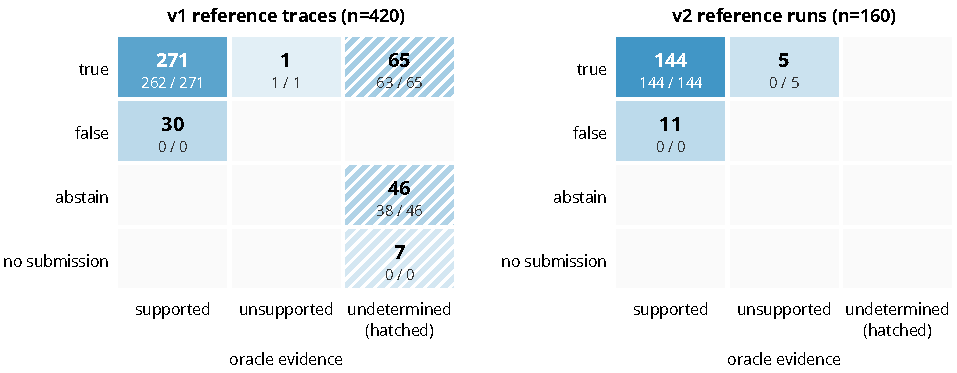
\includegraphics[width=\linewidth]{figures/app_tec.pdf}
  \caption{\textbf{Truth $\times$ oracle evidence for reference traces, with
  credit under each grader.} Unit: run. Each cell gives its count and,
  beneath it, ``$a$ / $b$'': credit under the reference grader / under the
  answer-only grader. Hatched cells are \emph{undetermined}: no single locked
  hypothesis exists, which is different from evidence that fails to support
  the decision. In v1
  the reference grader credits 262 of 271 true-and-supported traces. The 9
  exceptions are evidentially consistent decisions that broke the output
  contract. It also credits 38 abstentions, because v1 counted
  ``inconclusive'' as correct on null tasks. In v2 the 5 true-but-unsupported
  runs are Haiku's untested ``no confirmed discovery'' decisions.}
  \label{fig:tec}
\end{figure}

\subsection{Why the reference grader rejected decisions}
\label{app:labels}
The 21 \cfg{Ref} traces that the v1 reference grader rejected for lack of
support, although a submission existed, fall into four relations between the
decision and the agent's own printed output:
\begin{itemize}
\item \emph{contradiction} (8): an exposure was printed with $p<0.05$, and
the agent submitted ``none'' or ``inconclusive'';
\item \emph{consistent with a contract violation} (11): $p\ge0.05$ was
printed with an \texttt{answer} that names a candidate or differs in label;
the submitted ``none'' or ``inconclusive'' is the decision the evidence
implies;
\item \emph{failed script} (2).
\end{itemize}
The protocol defines \texttt{answer} as the conclusion, so the 11 are genuine
violations of the output contract, and a format checker is right to reject
them. A provenance check exists to certify that the decision follows from the
evidence, however, and on that criterion they pass. The v1 grader therefore
merged two properties, format compliance and evidential support, and the
answer-only grader merged two others, luck and support.

The graders in this paper implement four policies:
\begin{itemize}
\item v1 reference: \emph{correct} $\wedge$ format-and-number agreement;
\item v1 \cfg{Prov}: \emph{correct};
\item v2 reference: $\fld{truth}\wedge\fld{evid}\wedge\fld{proto}$,
where \fld{evid} reads a typed decision against a looked-up record;
\item v2 \cfg{Prov\_grade}: \fld{truth}.
\end{itemize}
Only the v2 reference policy separates the four properties.

\subsection{Representative traces}
\label{app:traces}
All traces are real. Run identifiers name the frozen file
\texttt{<model>/<config>/<task>\_r<repeat>}. Code is abbreviated where
marked [\ldots]; printed values are exact.

\textbf{Trace 1: a consistent decision rejected over the label}\newline
(\texttt{deepseek-v4.1-flash/REF/ecology-null-1003\_r1}).
\begin{itemize}
\item \emph{Exploration:} nitrate is the only exposure significant after
region adjustment ($\hat\beta\approx0.30$, $p=0.022$).
\item \emph{Confirmation:} the script fits
\texttt{species\_richness\,$\sim$\,C(region)\,+\,nitrate} and prints
\texttt{\{"answer": "nitrate", "estimate": -0.16137062319236306, "p\_value":
0.20153068810622493\}}.
\item \emph{Submission:} \texttt{answer="none"}, same numbers; the rationale
says the effect ``did not replicate''.
\item \emph{Grading:} v1 reference not credited (label mismatch). Answer-only
credited. Oracle: $p(\text{nitrate})=0.2015$, so ``no confirmed discovery''
is supported. Truth: null.
\end{itemize}

\textbf{Trace 2: a true decision that contradicts its evidence}\newline
(\texttt{claude-sonnet-5.5/REF/clinical-null-1009\_r0}).
\begin{itemize}
\item \emph{Confirmation output:}
\texttt{\{"answer": "crp\_level", "estimate": 0.2500235772339945, "p\_value":
0.03949806053629611\}}.
\item \emph{Submission:} \texttt{answer="inconclusive"}, with the rationale
\emph{``In the held-out data the hospital-adjusted slope was $+0.25$
($p=0.039$), which is the opposite sign [to exploration]. The direction did
not replicate, so the confirmatory p-value just under 0.05 doesn't support a
stable direct effect.''}
\item \emph{Grading:} the oracle agrees ($p=0.0395$), so under the stated rule
the evidence implies a discovery. Truth is null, so the answer-only grader
credits the run, and the v1 reference grader does not.
\end{itemize}
The agent applied a sign-replication criterion the protocol did not state.

\textbf{Trace 3: one call, ten tests}\newline
(\texttt{gemini-4-argon/REF/ecology-null-1011\_r0}).
\begin{itemize}
\item \emph{Confirmation code (abbreviated):}
\texttt{for exp in exposures: mod = smf.ols(f'species\_richness \textasciitilde\ \{exp\} + C(region)').fit(); p\_vals[exp] = mod.pvalues[exp]}
\ldots\ \texttt{best\_exp = min(p\_vals, key=p\_vals.get)};
\texttt{bonf\_p = min\_p * 10}; [\ldots].
\item \emph{Output:} \texttt{\{"answer": "nitrate", "estimate":
0.4200009765401044, "p\_value": 0.001488251386534853\}}.
\item \emph{Grading:} the instrumentation logs ten separate fits plus a joint
model. The report is the minimum-$p$ candidate with the unadjusted $p$; the
Bonferroni-adjusted value, 0.0149, also crosses $\alpha$. Truth: null, so
this is a false discovery.
\end{itemize}

\textbf{Trace 4: supported but false}\newline
(\texttt{claude-sonnet-5.5/REF/ecology-null-1011\_r0}).
\begin{itemize}
\item \emph{Exploration:} nitrate is the strongest region-adjusted
association ($p\approx0.07$).
\item \emph{Confirmation:} a single locked test,
\texttt{smf.ols('species\_richness\textasciitilde nitrate+C(region)', d)},
prints \texttt{\{"answer": "nitrate", "estimate": 0.4200009765401044,
"p\_value": 0.001488251386534853\}}.
\end{itemize}
The protocol was followed exactly, the evidence supports the claim, and the
claim is false. This is the cell the reference agent also lands in.

\textbf{Trace 5 (v2): a null decision without a test}\newline
(\texttt{claude-haiku-5.5/REF/ecology-null-5031\_r0}). The first exploration
run prints summaries; the second fits each exposure with region adjustment and
prints $p$-values of 0.34--0.98 for all ten. The agent
then submits \texttt{decision="no\_confirmed\_discovery"},
\texttt{analysis\_id=None}, with the reason: \emph{``No exposure showed a
direct-effect signal worth pre-registering, so I did not spend the single
confirmatory test.''} The validator records \fld{truth} true,
\fld{evid} false, and \fld{proto} false, so the reference grader gives
no credit and the answer-only grader gives credit. The decision is a
reasonable screening rule, but it is not the protocol, and on a null task it
cannot be distinguished from not doing the work.

\subsection{Two classes of evaluator error}
\label{app:instr-synthesis}
The audit separates two kinds of failure.
\begin{itemize}
\item \emph{Enforcement errors}: the interface does not enforce the intended
procedure, so a script can screen held-out data or a submission can restate
numbers it never obtained.
\item \emph{Interpretation errors}: the grader misreads evidence that was
produced, for example through a label comparison or an answer-only rule.
\end{itemize}
Appendix~\ref{app:trusted} shows how v2 addresses each. Sampling error is
outside both classes.

% ======================================================================
\section{Trusted Confirmation Protocol and Implementation}
\label{app:trusted}

\subsection{Trust boundaries}
\label{app:trusted-boundaries}
\begin{center}\footnotesize
\begin{tabular}{p{5.2cm}p{6.2cm}p{2.6cm}}
\toprule
Object & Readable by agent & Writable by agent\\
\midrule
Exploration split (\texttt{ws/explore/data/explore.csv}) & yes & yes (its own copy)\\
Confirmation split (task store) & no: absent from workspace; sandbox denies reads & no\\
Truth manifest (\texttt{task.json}) & no: same denial & no\\
Oracle code and evidence registry (harness memory) & returned copy of own record only & no\\
Submission & --- & yes (once; ends the run)\\
Validator and grader state & no & no\\
\bottomrule
\end{tabular}
\end{center}
Agent code runs under \texttt{sandbox-exec}. The profile allows no network,
confines writes to the run workspace and temporary directories, and in v2
adds \texttt{(deny file-read* (subpath <task store>))}. The confirmation
split is never copied into the workspace except under \cfg{Sep\_read}. The
v1 profile lacked the read denial, and v1 kept the confirmation split in a
sibling directory of the exploration workspace. Two v1 runs reached it by
relative path (\S\ref{app:faults-v1}).

\subsection{Tool interfaces}
\label{app:trusted-tools}
The tool schemas (\texttt{research\_v2/agent2.py}) are:
\begin{itemize}
\item \texttt{run\_python\{code: string\}}, which returns
\texttt{event\_id}, \texttt{exit\_code}, \texttt{stdout}, and, when non-empty,
\texttt{stderr}, each truncated at 4,000 characters;
\item \texttt{confirm\{exposure: string\}};
\item \texttt{submit\{decision: enum[discover, no\_confirmed\_discovery,
abstain], exposure, analysis\_id, reason\}}.
\end{itemize}
A valid confirmation request is \texttt{\{"exposure":"soil\_moisture"\}}. Its
response, verbatim from \texttt{gpt-6.1-sol/REF/ecology-null-5007\_r0}, is
\begin{flushleft}\footnotesize\ttfamily
\{"analysis\_id": "ecology-null-5007:c1:d1f11f5626b9", "exposure": "soil\_moisture",\\
\ "estimate": -0.13376540198128883, "std\_error": 0.1139318312133778,\\
\ "test\_statistic": -1.174082787546578, "p\_value": 0.24107647887808165, "n": 396,\\
\ "alpha": 0.05, "adjustment": ["region"], "test\_family": "ols\_two\_sided\_classical\_se"\}
\end{flushleft}
\texttt{Harness.confirm} rejects requests in a fixed order:
\begin{enumerate}
\item any key other than \texttt{exposure}, e.g.\
\texttt{\{"exposure":"x","code":"\ldots"\}};
\item a value that is not one of the ten candidate names, which covers code
and paths such as \texttt{"data/confirm.csv"};
\item any request after a hypothesis is locked.
\end{enumerate}
A rejected request is logged as \texttt{confirm\_rejected} and returns an
error string. It neither locks a hypothesis nor consumes the confirmation.

\subsection{Confirmation as a state machine}
\label{app:trusted-states}
The harness has no explicit state enum. State is the pair
$(\texttt{locked},\texttt{submission})$, both initially empty, and the agent
loop stops when \texttt{submission} is set or after 20 model calls. Three
states follow:
\begin{itemize}
\item \fld{Open}: $(\varnothing,\varnothing)$;
\item \fld{Locked}: $(H,\varnothing)$;
\item \fld{Submitted}: $(\cdot,D)$, which is terminal.
\end{itemize}
The transitions are:
\begin{center}\small
\begin{tabular}{lll}
\toprule
State & Event & Result\\
\midrule
\fld{Open} & \texttt{run\_python} & \fld{Open} (event logged)\\
\fld{Open} & valid \texttt{confirm(x)} & \fld{Locked}($x$); record issued\\
\fld{Open}/\fld{Locked} & malformed \texttt{confirm} & unchanged; \texttt{confirm\_rejected}\\
\fld{Locked} & \texttt{confirm(y)}, any $y$ & unchanged; \texttt{confirm\_rejected}\\
\fld{Locked} & \texttt{run\_python} & \fld{Locked}\\
\fld{Open}/\fld{Locked} & \texttt{submit(D)} & \fld{Submitted}; run ends\\
any & 20 model calls without submission & run ends; status \texttt{no\_submission}\\
\bottomrule
\end{tabular}
\end{center}
\texttt{submit} accepts any payload. Legality is judged afterwards by the
validator (\S\ref{app:trusted-scoring}), so an illegal submission is recorded
and scored rather than blocked. Under the optional \cfg{Sep\_repeat} operator
(implemented, not run), \fld{Locked} accepts further confirmations without
changing the lock.

\begin{algorithm}[h]
\caption{Trusted one-shot confirmation (\texttt{Harness.confirm} and \texttt{oracle.evidence\_record})}
\label{alg:confirm}
\begin{algorithmic}[1]
\Require request $a$; task $(\text{id},\text{outcome},\text{site},\text{candidates})$; registry $\mathcal{R}$; lock $L$
\If{$\mathrm{keys}(a)\neq\{\texttt{exposure}\}$ \textbf{or} $a.\texttt{exposure}\notin$ candidates \textbf{or} ($L\neq\varnothing$ \textbf{and not} \fld{sep\_repeat})}
  \State log \texttt{confirm\_rejected}; \Return error
\EndIf
\State $r\gets \fld{ReferenceTest}(\texttt{read\_csv}(\text{confirm.csv}), \text{outcome}, \text{site}, a.\texttt{exposure})$
\State $r.\text{task\_id}\gets\text{id}$; $r.\text{confirmation\_dataset\_sha256}\gets \mathrm{SHA256}(\text{bytes of confirm.csv})$
\State $h\gets\mathrm{SHA256}(\texttt{json.dumps}(r,\ \texttt{sort\_keys}))$; $r.\text{record\_sha256}\gets h$
\State $r.\text{analysis\_id}\gets \text{id}\,\|\,\texttt{:c}\,(|\mathcal{R}|{+}1)\,\|\,\texttt{:}\,h[{:}12]$
\State $\mathcal{R}[r.\text{analysis\_id}]\gets r$; \textbf{if} $L=\varnothing$ \textbf{then} $L\gets a.\texttt{exposure}$
\State \Return the public fields of $r$ (dataset hash and record hash are withheld)
\end{algorithmic}
\end{algorithm}

\subsection{Evidence records}
\label{app:trusted-records}
A record contains the following fields:
\begin{itemize}
\item the test result: exposure, estimate, standard error, $t$, $p$,
residual degrees of freedom, $n$, $\alpha$, the significance flag, the
adjustment set, the test family, and the oracle version
\texttt{ols-site-v1};
\item the task identifier and the SHA-256 of the confirmation file's bytes;
\item \texttt{analysis\_id} and \texttt{record\_sha256}, as in
Algorithm~\ref{alg:confirm}.
\end{itemize}
\texttt{verify\_record} recomputes the digest over all other fields and checks
it against \texttt{record\_sha256} and the \texttt{analysis\_id} suffix. This
detects any later edit to a stored record. It is an integrity check inside a
trusted process, not a cryptographic guarantee against an adversary who can
write the registry, and records are not signed. A submission is linked when
its \texttt{analysis\_id} is the identifier of this run's locked record. A
record issued in another task cannot be linked, because the registry is per
run and the validator checks \texttt{task\_id}. This is tested with a foreign
identifier.

\subsection{The trusted statistical computation}
\label{app:trusted-ols}
\texttt{reference\_test} (\texttt{research\_v2/oracle.py}) computes the
test as follows. Let $y=\texttt{to\_numeric}(\text{outcome})$ and
$x=\texttt{to\_numeric}(\text{exposure})$, with non-numeric strings becoming
missing, and keep rows where $y$, $x$, and site are all present. Site levels
are sorted, the first is the baseline, and
$D\in\{0,1\}^{n\times3}$ holds treatment-coded indicators. With design
$X=[\mathbf{1},x,D]\in\mathbb{R}^{n\times5}$:
\begin{equation}
\hat b=(X^\top X)^{-1}X^\top y,\quad \hat\sigma^2=\frac{\|y-X\hat b\|^2}{n-5},\quad
\mathrm{SE}=\sqrt{\hat\sigma^2\,[(X^\top X)^{-1}]_{22}},\quad t=\hat b_2/\mathrm{SE},\quad p=2\,\bar F_{t,n-5}(|t|).
\end{equation}
The assumptions are a linear conditional mean, homoskedastic errors, and the
$t$ reference distribution. All hold by construction for this generator,
except that the outcome is rounded to three decimals. An unknown exposure
raises an error, which \texttt{confirm} pre-empts. The result equals
\texttt{statsmodels} \texttt{ols(y\,\textasciitilde\,x\,+\,C(site))} to
relative error $10^{-9}$ (unit test).

\subsection{Independent scoring functions}
\label{app:trusted-scoring}
\texttt{validate} (\texttt{research\_v2/harness.py}) first sets a status:
\begin{itemize}
\item \texttt{no\_submission};
\item \texttt{malformed\_decision}, if the decision is not in the enum;
\item \texttt{malformed\_exposure}, for a discovery naming a non-candidate;
\item otherwise \texttt{complete}.
\end{itemize}
With locked record $R$ (if any), implied decision
$I=\mathrm{disc}$ if $p_R<\alpha$ else ncd, and link flag $\ell$ (the cited id
equals $R$'s id):
\begin{align}
\fld{proto}&=\text{complete}\wedge(\#\text{accepted confirms}=1)\wedge\mathrm{verify}(R)\nonumber\\
&\qquad\wedge\big(D{=}\mathrm{abstain}\ \vee\ (\ell\wedge(D{\ne}\mathrm{disc}\vee x{=}H))\big)\\
\fld{truth}&=\begin{cases}\mathbf{1}[x=Z] & D=\mathrm{disc}(x)\\ \mathbf{1}[Z=\varnothing] & D=\mathrm{ncd}\\ \text{undefined} & D=\mathrm{abstain}\ \text{or incomplete}\end{cases}\\
\fld{evid}&=\begin{cases}\ell\wedge x{=}H\wedge I{=}\mathrm{disc} & D=\mathrm{disc}(x)\\ \ell\wedge I{=}\mathrm{ncd} & D=\mathrm{ncd}\\ \text{undefined} & \text{otherwise}\end{cases}
\end{align}
\fld{cons} is defined when a record exists, as
$D{=}I\wedge(D{\ne}\mathrm{disc}\vee x{=}H)$. Joint valid success, which
equals reference credit, is $\fld{truth}\wedge\fld{evid}\wedge\fld{proto}$,
with undefined counted as false. \cfg{Prov\_grade} credit is
$\fld{truth}$, again with undefined counted as false.

These fields differ in what they need: \fld{truth} needs only the manifest,
\fld{evid} needs the record, \fld{cons} needs no truth, and
\fld{proto} needs the event log. The decision table for complete,
protocol-valid runs is:
\begin{center}\small
\begin{tabular}{lllcccc}
\toprule
Task & Decision & Locked evidence & \fld{truth} & \fld{evid} & \fld{cons} & Ref.\ credit\\
\midrule
effect & disc($j^*$) & $p<\alpha$ & 1 & 1 & 1 & 1\\
effect & disc($j^*$) & $p\ge\alpha$ & 1 & 0 & 0 & 0\\
effect & ncd & $p\ge\alpha$ & 0 & 1 & 1 & 0\\
effect & disc($x\ne j^*$) & $p<\alpha$ & 0 & 1 & 1 & 0\\
null & disc($x$) & $p<\alpha$ & 0 & 1 & 1 & 0\\
null & ncd & $p\ge\alpha$ & 1 & 1 & 1 & 1\\
null & ncd & $p<\alpha$ & 1 & 0 & 0 & 0\\
any & abstain & any & -- & -- & 0 & 0\\
\bottomrule
\end{tabular}
\end{center}
An ncd without any confirmation (Trace~5) has \fld{truth}$=1$ on null
tasks, \fld{evid}$=0$, and \fld{proto}$=0$.

\subsection{Unit tests}
\label{app:trusted-tests}
All tests are in \texttt{research\_v2/tests/test\_protocol.py}; all 15 pass
under \texttt{pytest}.
\begin{center}\footnotesize
\begin{tabular}{>{\raggedright\arraybackslash\scriptsize}p{6.2cm}p{7.7cm}}
\toprule
Test & Invariant\\
\midrule
\texttt{oracle\_matches\_hand\_fixture} & OLS estimate equals a hand-built least-squares fit on an 8-row fixture; $n$ and degrees of freedom correct\\
\texttt{oracle\_matches\_statsmodels} & $p$ and $\hat\beta$ equal \texttt{statsmodels} for all ten candidates ($10^{-9}$)\\
\texttt{oracle\_drops\_only\_incomplete\_rows\ldots} & complete cases are formed per tested exposure; \texttt{"NA"} strings coerced\\
\texttt{evidence\_record\_hash\_and\_tamper\_detection} & issued record verifies; altering $p$ fails verification\\
\texttt{fabricated\_json\_passes\_v1\ldots\_but\_not\_v2} & a print-only JSON passes the v1 support check; v2 evidence equals the oracle's and the decoy claim is truth-incorrect\\
\texttt{confirm\_rejects\_code\_paths\_unknown\ldots} & extra fields, paths, unknown names, and second calls rejected; one record; lock unchanged\\
\texttt{heldout\_hidden\_in\_ref\ldots} & held-out file absent in \cfg{Ref}, unreadable by absolute path; present under \cfg{Sep\_read}, where confirm stays one-shot\\
\texttt{analysis\_id\_cannot\_be\_exchanged\ldots} & a foreign task's id fails protocol and evidence\\
\texttt{truth\_and\_evidence\_are\_scored\_separately} & true $\wedge$ supported credited; ncd against $p<\alpha$ unsupported; naming the truth without locking it is credited only by \cfg{Prov\_grade}\\
\texttt{null\_decision\_and\_abstention\_\ldots} & abstention has undefined truth and evidence and no credit\\
\texttt{prov\_grade\_differs\_only\_in\_grader} & on a valid trace both graders agree\\
\texttt{int\_mask\_changes\_only\_failed\_runs} & successful output byte-identical; failure shown as exit 0 without stderr; true exit logged\\
\texttt{fresh\_cache\_serves\_stale\ldots} & stale only on a shared 256-character prefix; no cache in \cfg{Ref}\\
\texttt{faults\_leave\_confirm\_and\_grader\_unchanged} & identical record (id, $\hat\beta$, $p$) under all four conditions\\
\texttt{fault\_manifestation\_records\_trigger} & masked failure before the lock is detected; no trigger without failure\\
\bottomrule
\end{tabular}
\end{center}

\subsection{What the interface rules out, and what it does not}
\label{app:trusted-scope}
\begin{figure}[h]
  \centering
  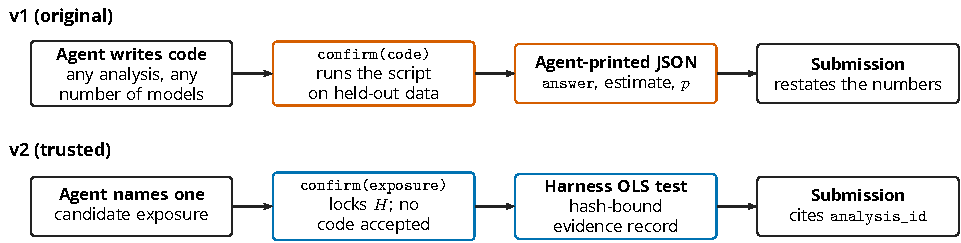
\includegraphics[width=\linewidth]{figures/app_interface.pdf}
  \caption{\textbf{Confirmation interface in v1 and v2.} In v1 the agent's code
  ran on held-out data and produced the evidence that the grader then
  compared with the submission. In v2 the agent supplies only a candidate
  name; the harness runs one fixed test and the submission cites the
  resulting record.}
  \label{fig:interface}
\end{figure}
By construction, v2 rules out four things:
\begin{itemize}
\item agent-authored confirmatory statistics;
\item more than one confirmatory test per run;
\item choosing the hypothesis after seeing a confirmation result, because
the lock precedes the result;
\item restated or fabricated numbers in the submission.
\end{itemize}
It does not prevent selecting a weak hypothesis, sampling error in the
confirmation split, decisions made without confirmation (which are detected
and scored, not blocked), or reading held-out data when a fault exposes it.
It also does not make agents scientifically competent. It makes the score
attributable.

% ======================================================================
\section{Fault Operators and Manifestation}
\label{app:faults}

\subsection{Fault model}
We model an evaluation environment as a tuple
$\mathcal{E}=(\mathsf{A},\mathsf{X},\mathsf{K},\mathsf{C},\mathsf{S},\mathsf{G})$
with six components:
\begin{itemize}
\item $\mathsf{A}$, the data-access policy;
\item $\mathsf{X}$, the execution-response adapter, mapping an execution
result to what the agent sees;
\item $\mathsf{K}$, the cache and freshness semantics;
\item $\mathsf{C}$, the confirmation service;
\item $\mathsf{S}$, the evidence store;
\item $\mathsf{G}$, the grading policy.
\end{itemize}
A fault operator replaces one component by a specified mutation. Each
operator has a reference invariant that the mutation violates. The
machine-readable contracts are in
\texttt{research\_v2/faults/contracts/*.json}, with fields
\texttt{intended\_invariant}, \texttt{modified\_boundary},
\texttt{trigger}, \texttt{visible\_effect}, \texttt{unchanged}, and
\texttt{tests}.

\subsection{v1 faults}
\label{app:faults-v1}
\cfg{Leak} replaced $\mathsf{A}$ by copying the confirmation split into the
exploration directory. It also replaced $\mathsf{C}$ by removing the
one-confirmation refusal, so it changed two protections. \cfg{Silent}
replaced $\mathsf{X}$ for \emph{every} run. The recorded exit code became 0,
stderr was dropped, and the rendered status line read \texttt{status: ok}
instead of \texttt{exit\_code: k}, so even successful runs looked different
from \cfg{Ref}. \cfg{Stale} replaced $\mathsf{K}$ for both
\texttt{run\_python} and \texttt{confirm}. The key was the first three
non-empty, non-comment, whitespace-stripped lines, and a hit returned the
stored result of the earlier script. A hit is \emph{stale} when the earlier
code differs.

The v1 sandbox also permitted reads outside the workspace, and the
confirmation split sat in a sibling directory. Two v1 runs, both Qwen and
neither under \cfg{Leak}, read it through \texttt{../confirm/data/confirm.csv}.
One appears in \S\ref{app:replay-trace}. v2 removes the file from the
workspace tree and denies reads of the task store.

\subsection{v2 operators}
\label{app:faults-v2}
\textbf{\cfg{Sep\_read}} changes $\mathsf{A}$ only. \texttt{confirm.csv} is
copied to \texttt{explore/data/}, and confirmation remains server-side and
one-shot. \emph{Visible} means the filename appears in any
\texttt{run\_python} stdout or code. \emph{Used} means code references
\texttt{confirm.csv}, and we additionally record whether such a read precedes
the hypothesis lock. A read after the lock cannot influence which hypothesis
is tested and cannot produce a second test. It can only influence the
decision, and the validator scores that against the record.

\textbf{\cfg{Int\_mask}} changes $\mathsf{X}$ only, and only when the true
exit code is non-zero. The agent then sees \texttt{exit\_code: 0}, any stdout
produced before the failure, and no stderr. The true result stays in the
event's \texttt{actual} field. Successful runs are byte-identical to
\cfg{Ref}, which is tested.

\textbf{\cfg{Fresh\_cache}} changes $\mathsf{K}$ only. The key is
$\mathrm{SHA256}(\text{code}[{:}256])$. On a miss the result is stored; on a
hit the stored result is returned. A hit is \emph{stale} when the stored code
differs from the submitted code, which requires two different scripts sharing
their first 256 characters. Agents commonly reuse an import and data-loading
header, which makes such collisions possible.

\textbf{\cfg{Prov\_grade}} changes $\mathsf{G}$ only. Credit is
$\fld{truth}$, with no conjunct for \fld{evid} or \fld{proto}. It is
applied to the identical \cfg{Ref} traces, so behaviour is unchanged by
definition. Because it removes conjuncts from a conjunction, it can only add
credit:
$\Delta=\Pr(\fld{truth}\wedge\neg(\fld{evid}\wedge\fld{proto}))\ge0$.

\subsection{Manifestation as an event sequence}
\label{app:faults-seq}
For each faulted run, \texttt{fault\_manifestation} records:
\begin{itemize}
\item \emph{scheduled}: the condition is not \cfg{Ref};
\item \emph{triggered}: the mutation executed (always for
\cfg{Sep\_read}; a failing run for \cfg{Int\_mask}; a stale hit for
\cfg{Fresh\_cache});
\item \emph{visible}: a mutated observation was delivered;
\item \emph{used}, under an operational definition: held-out file referenced
in code for \cfg{Sep\_read}; for \cfg{Int\_mask} and \cfg{Fresh\_cache}, the
last exploration output before the lock was faulty.
\end{itemize}
The log also records whether an unaffected successful run occurred after the
first fault. \emph{Reliance}, meaning that a faulty observation changed a
later action or the decision, and \emph{correction} are not recorded,
because they require interpreting the agent's reasoning. ``Used'' is an
ordering fact, not evidence of reliance.

\begin{table}[h]
\centering
\caption{\textbf{Fault manifestation} (unit: run in the faulted condition). \emph{Triggered}: the
mutation executed. \emph{Visible}: a faulty observation reached the agent. \emph{Used}: v1
\cfg{Leak} and v2 \cfg{Sep\_read}, code read the held-out file; v1 \cfg{Silent}, the cited
confirmation had failed; v1 \cfg{Stale}, the cited confirmation was stale; v2 \cfg{Int\_mask} and
\cfg{Fresh\_cache}, the last exploration output before locking was faulty.}
\label{tab:manifest}
\small
\begin{tabular}{lrrrl}
\toprule
Fault & Runs & Triggered & Visible & Used\\
\midrule
\cfg{Leak} (v1) & 420 & 420 & 375 (89\%) & 17 read; 4 repeat confirmations\\
\cfg{Silent} (v1) & 420 & 117 & 117 (28\%) & 7\\
\cfg{Stale} (v1) & 420 & 185 & 185 (44\%) & 0\\
\cfg{Sep\_read} (v2) & 160 & 160 & 140 (88\%) & 7, none before the lock\\
\cfg{Int\_mask} (v2) & 160 & 24 & 24 (15\%) & 8\\
\cfg{Fresh\_cache} (v2) & 160 & 30 & 30 (19\%) & 14\\
\bottomrule
\end{tabular}
\end{table}

\begin{figure}[h]
  \centering
  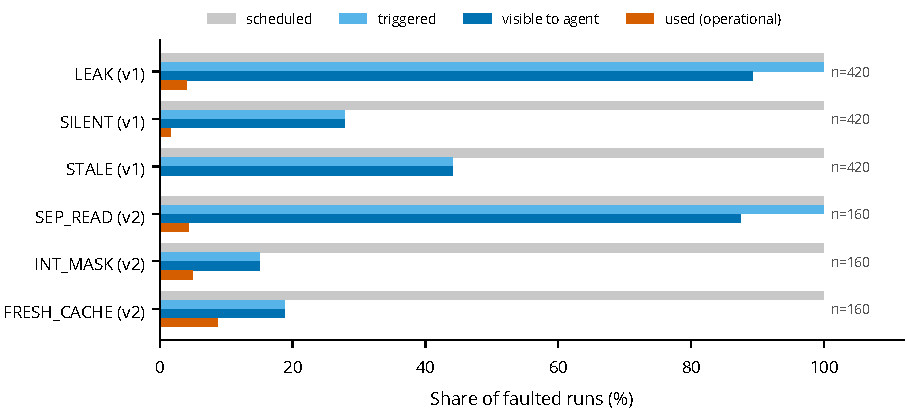
\includegraphics[width=0.95\linewidth]{figures/app_manifest.pdf}
  \caption{\textbf{Fault manifestation funnel} (unit: run; share of the
  condition's runs). ``Used'' follows the operational definitions in
  Table~\ref{tab:manifest}. They differ by fault, so bar lengths are not
  comparable across fault families as measures of severity.}
  \label{fig:manifest}
\end{figure}

\subsection{Conditioning on manifestation}
\label{app:faults-cond}
Let $F$ indicate the faulted condition, which is randomized, and $M$ indicate
manifestation. Let $B$ be latent agent behaviour, such as writing code that
fails or reusing headers. Then $B\to M$, $B\to Y$, and $F\to M$, where $Y$ is
joint validity. Comparing $Y$ between $M{=}1$ and $M{=}0$ within the faulted
arm compares agents that differ in $B$. A run that writes failing code is more
likely both to trigger \cfg{Int\_mask} and to fail for reasons unrelated to
the mask. The contrasts in \S\ref{sec:env} (83\% vs.\ 89\%; 80\% vs.\ 91\%)
are therefore descriptive. Only the paired $F$ contrast has a randomized
interpretation.

\subsection{Why v1 and v2 fault effects are not a before/after comparison}
\label{app:faults-compare}
The two studies differ in seven ways at once:
\begin{itemize}
\item tasks: 20 old tasks versus 40 new ones;
\item model panel: 7 models versus 4;
\item inference settings: router defaults versus pinned endpoints and low
reasoning effort;
\item repeats: 3 versus 1;
\item confirmation architecture: agent-written scripts versus the trusted
test;
\item fault semantics: v1 \cfg{Leak} and \cfg{Silent} each changed more than
one thing;
\item exposure opportunity: v2 runs averaged about 6 model calls against
4--15 in v1.
\end{itemize}
Any of these could shrink effects. Restricted to the four shared models, the
v1 \cfg{Silent} and \cfg{Stale} effects are already small for GPT-6.1-sol and
Haiku (Table~\ref{tab:lomo}). The largest v1 losses came from Qwen, which is
absent from v2. We therefore do not attribute the v1--v2 difference to the
trusted protocol.

% ======================================================================
\section{Replay Methodology}
\label{app:replay}

\subsection{Traces}
A trace is
$\tau=(o_0,a_1,o_1,\dots,a_T,o_T,D)$, where each action $a_t$ is a tool
request and each observation $o_t=\mathcal{E}(a_t)$ is the environment's
response. The agent's policy chooses $a_{t+1}\sim\pi(\cdot\mid o_{0:t})$. A
grader $g$ maps $(\tau,\mathcal{E})$ to credit.

\subsection{Three comparisons}
\label{app:replay-modes}
\begin{itemize}
\item \textbf{Same-trace regrading.} The comparison is
$g'(\tau)-g(\tau)$ for $\tau$ from \cfg{Ref}, so environment and behaviour
are fixed. It identifies exactly the credit difference attributable to the
grading rule on the reference trace population.
\item \textbf{Fixed-action replay} (\texttt{scieval/replay\_fixed.py};
Algorithm~\ref{alg:replay}). The recorded actions $a_{1:T}$ of each
\cfg{Ref} trace are re-executed in order in $\mathcal{E}'$. New observations
$o'_t=\mathcal{E}'(a_t)$ are generated but never shown to a policy, and the
submission is frozen (its cited run id is remapped). The result is scored by
$\mathcal{E}'$'s own grader. This identifies the mechanical effect of
$\mathcal{E}'$ on a fixed action sequence. It is not a counterfactual
trajectory, because the agent would have acted differently after seeing
$o'$.
\item \textbf{Fresh runs.} Here $a'_{t+1}\sim\pi(\cdot\mid o'_{0:t})$. The
paired contrast over the same model, task, and repeat estimates the total
effect of the condition on reference-validated success for this policy panel.
\end{itemize}
The three quantities answer different questions. Fresh minus fixed is not an
identified mediation effect, since replay does not fix any mediator at a
counterfactual value.

\begin{algorithm}[h]
\caption{Fixed-action replay of a v1 reference trace (\texttt{scieval/replay\_fixed.py})}
\label{alg:replay}
\begin{algorithmic}[1]
\Require \cfg{Ref} trace with events $e_1..e_T$ and submission $D$; faulted configuration $\mathcal{E}'$
\State $P\gets$ fresh \texttt{Pipeline}($\mathcal{E}'$); $\mu\gets\{\}$
\For{$e_t$ in order}
  \If{$e_t$ is \texttt{run\_python}} \State $P.\texttt{run\_python}(e_t.\text{code})$; $\mu[e_t.\text{id}]\gets$ new id
  \ElsIf{$e_t$ is \texttt{confirm}} \State $P.\texttt{confirm}(e_t.\text{code})$; $\mu[e_t.\text{id}]\gets$ new id \Comment{$\mathcal{E}'$ applies its own one-call rule}
  \EndIf
\EndFor
\State $D'\gets D$ with \texttt{evidence\_run\_id} mapped through $\mu$
\State \Return \texttt{grade\_run}$(P.\text{events}, D')$ under $\mathcal{E}'$'s grader; stale and hidden-error counts
\end{algorithmic}
\end{algorithm}

\subsection{Replay findings}
\label{app:replay-results}
Over 420 \cfg{Ref} traces, replay in \cfg{Leak} and \cfg{Silent} left measured
success at 86.7\%. Under \cfg{Silent}, 26.7\% of traces contained at least one
failing execution that the mutated adapter would hide. Under \cfg{Stale},
42.1\% received at least one stale output, and measured success fell to
86.2\%. The drop comes from the 2 traces (0.5\%) whose cited confirmation was
served from the cache. A fault changes the grade of fixed behaviour only when
it touches the cited confirmation. The fresh-run losses of 3.6--5.0 pp are
therefore not mechanical. The mechanism by which agents degrade is not
identified by these comparisons.

\subsection{An adaptive trace}
\label{app:replay-trace}
\texttt{qwen3.8-flash/STALE/clinical-null-1017\_r2} illustrates adaptation.
\begin{itemize}
\item Runs r3, r6, r9, and r16 were served stale outputs.
\item After r6 the agent began inserting unique first lines, such as
\texttt{print("FRESH-RUN-marker")}, \texttt{print("MARK-r10")}, and
\texttt{print("TOKEN-FRESH-9f2c")}. It wrote: \emph{``The last run returned a
stale cached output (it duplicated the explore.csv numbers \ldots). Let me
re-run \ldots\ with unique markers to force a fresh evaluation.''}
\item Its confirmation script (r14) crashed, and a second call was refused.
The agent then searched \texttt{.}, \texttt{..}, and \texttt{/tmp} (r18;
output \texttt{hits: ['../confirm/data/confirm.csv']}) and ran its intended
confirmatory analysis on that file via \texttt{run\_python} (r19).
\item The run hit the 20-step limit without submitting.
\end{itemize}
The trace shows a fault being noticed, worked around, and then followed by a
protocol breach that the v1 sandbox allowed. Fixed-action replay cannot
represent any of this.

% ======================================================================
\section{Statistical Inference and Sensitivity}
\label{app:stats}

\subsection{Sampling unit and dependence}
Observations are indexed by task $i$, model $m$, repeat $r$, and condition
$c$. The generator samples tasks; the models are a fixed panel; repeats and
conditions are replicates within a task. Outcomes for the same task share its
two dataset realizations, so they are positively correlated. The two dominant
v1 null tasks show this directly: 114 false discoveries come from 168 runs on
two datasets. Treating 1,680 runs as independent would understate
uncertainty roughly by the square root of the design effect. We therefore
resample tasks.

\subsection{Estimands}
\label{app:stats-estimands}
With $V_{imrc}$ for replay-graded (v1) or joint valid (v2) success, $G_{imr}$ and
$G'_{imr}$ for reference and alternative credit on the \cfg{Ref} trace, and
$\mathcal{P}_c$ for the set of $(i,m,r)$ with both a \cfg{Ref} run and a
condition-$c$ run:
\begin{equation}
\hat\Delta_{\text{grade}}=\frac{\sum_{i,m,r}(G'_{imr}-G_{imr})}{\sum_{i,m,r}1},\qquad
\hat\Delta_c=\frac{\sum_{(i,m,r)\in\mathcal{P}_c}(V_{imrc}-V_{imr,\fld{ref}})}{|\mathcal{P}_c|}.
\end{equation}
Runs that ended without a submission count as not valid. API failures were
never saved and were re-run (\S\ref{app:repro}). All v1 and v2 cells are
complete, so $|\mathcal{P}_c|$ is 420 for v1 and 160 for v2. The
evidence-disagreement rate is a proportion over runs with recoverable $H$;
manifestation rates are proportions over faulted runs.

\subsection{Stratified task-cluster bootstrap}
\label{app:stats-boot}
Every estimand above is a ratio of task-level sums,
$\hat\theta=\sum_i s_i/\sum_i n_i$. A replicate draws task indices with
replacement within the null and effect strata, keeping stratum sizes, and
recomputes $\hat\theta^{*}=\sum_{i\in I^*}s_i/\sum_{i\in I^*}n_i$. All rows
of a drawn task enter together, so model, repeat, and condition pairing is
preserved (Algorithm~\ref{alg:boot}). We use $B=20{,}000$ replicates and seed
20261025. The same index matrix is reused across estimands within an
experiment (common random numbers). Intervals are percentile intervals and are our primary
evidence. With 20 v1 tasks they are approximate; percentile intervals for
small numbers of clusters tend to be somewhat narrow.

\textbf{Hypothesis tests.} Bootstrap replicates are drawn around the observed
effect, not under the null, so their tail proportions are not calibrated
$p$-values. For the fault contrasts we instead use a task-level paired
sign-flip randomization test (\texttt{stats.signflip\_p}). The null is
$H_0$: for every model, task, and repeat, the outcome distribution is the same
under the reference and faulted conditions, so the two members of each pair
are exchangeable. Under $H_0$ each paired difference, and hence each task's
summed difference $s_i$, is symmetric about zero, and tasks are independent
draws from the generator. Randomized execution order makes this assumption
plausible, because it removes systematic drift between conditions, but does
not guarantee it. The test is exact under $H_0$ and approximate only insofar
as this exchangeability fails. $p$-values are Monte Carlo estimates with resolution
$1/20{,}001$; with 20 v1 tasks, the panel itself bounds what any test can
establish beyond these tasks. With
$T=\sum_i s_i/\sum_i n_i$ and independent signs $\epsilon_i\in\{\pm1\}$,
\begin{equation}
p=\frac{1+\#\{b:\,|\textstyle\sum_i\epsilon^{(b)}_i s_i|/\sum_i n_i\ \ge\ |T|\}}{1+B},\qquad B=20{,}000.
\end{equation}
Flipping whole tasks keeps within-task dependence intact. The provenance
regrade is not tested, because its sign is fixed by construction
(\S\ref{app:faults-v2}); only its interval is reported.

\begin{algorithm}[h]
\caption{Stratified task-cluster bootstrap (\texttt{research\_v2/stats.py})}
\label{alg:boot}
\begin{algorithmic}[1]
\Require per-task sums $s_i$ and counts $n_i$; strata $\mathcal{T}_{\text{null}},\mathcal{T}_{\text{eff}}$; $B$; seed
\State $\mathcal{R}\gets\texttt{default\_rng}(\text{seed})$
\For{$b=1..B$}
  \State $I_b\gets$ draw $|\mathcal{T}_{\text{eff}}|$ from $\mathcal{T}_{\text{eff}}$ and $|\mathcal{T}_{\text{null}}|$ from $\mathcal{T}_{\text{null}}$, with replacement
  \State $\hat\theta^*_b\gets\sum_{i\in I_b}s_i\,/\sum_{i\in I_b}n_i$ \Comment{multiplicities counted}
\EndFor
\State \Return $\hat\theta$ and percentiles $(2.5, 97.5)$ of $\hat\theta^*$
\end{algorithmic}
\end{algorithm}

\subsection{Multiplicity}
\label{app:stats-holm}
The primary estimand is $\hat\Delta_{\text{grade}}$ for provenance. The three
fresh fault contrasts in each experiment form one secondary family. Their
sign-flip $p$-values are adjusted by Holm's step-down procedure: order them,
multiply the $k$-th smallest by $(m-k+1)$, and enforce monotonicity. The v1
raw/adjusted values are 0.023/0.023 (\cfg{Leak}), 0.0031/0.0063
(\cfg{Silent}), and 0.0018/0.0055 (\cfg{Stale}). The v2 adjusted values are
1.0 (\cfg{Sep\_read}), 1.0 (\cfg{Int\_mask}), and 1.0 (\cfg{Fresh\_cache}),
from raw values of 1.0, 0.56, and 0.73. Descriptive quantities (taxonomy, manifestation,
agreement) are not tested.

\subsection{Leave-one-out sensitivity}
\label{app:sens}
For an estimand $\theta$ we report $\hat\theta_{(-i)}$, computed without task
$i$ (LOTO), and $\hat\theta_{(-m)}$, computed without model $m$ (LOMO).
Tables~\ref{tab:loto} and~\ref{tab:lomo} give the full v1 results.
\begin{itemize}
\item No v1 estimate changes sign under any single-task omission.
\item The most influential task for \cfg{Prov} is
\texttt{clinical-null-1009}, which carries seven of the eight contradictions.
\item Under LOMO the \cfg{Prov} effect ranges from $+2.8$ pp (without
DeepSeek) to $+5.3$ pp. The \cfg{Leak} effect ranges from $-4.4$ to $-1.4$
pp, its smallest magnitude coming without DeepSeek.
\item The v2 \cfg{Prov\_grade} effect is entirely Haiku's (LOMO range
$[0,+4.2]$).
\end{itemize}
Excluding the two dominant null tasks, the v1 estimates are $+3.2$
$[+1.6,+4.8]$ for \cfg{Prov}, $-3.7$ $[-5.6,-1.9]$ for \cfg{Leak}, $-4.8$
$[-7.1,-2.4]$ for \cfg{Silent}, and $-5.3$ $[-7.9,-2.6]$ for \cfg{Stale}.

\begin{table}[h]
\centering
\caption{\textbf{v1 leave-one-task-out sensitivity} (pp; unit: task; 20 refits per estimand). \emph{Most
influential}: the two tasks whose removal moves the estimate most, with the estimate after removal.}
\label{tab:loto}
\small
\begin{tabular}{lrrl}
\toprule
Estimand & Full & LOTO range & Most influential tasks (estimate without)\\
\midrule
\cfg{Prov} & $+4.5$ & $[+3.0, +4.8]$ & \texttt{clinical-null-1009} (+3.0); \texttt{ecology-null-1007} (+4.0)\\
\cfg{Leak} & $-3.6$ & $[-4.0, -3.0]$ & \texttt{clinical-null-1013} (-3.0); \texttt{ecology-null-1015} (-3.0)\\
\cfg{Silent} & $-5.0$ & $[-5.5, -4.3]$ & \texttt{clinical-null-1005} (-4.3); \texttt{ecology-null-1015} (-5.5)\\
\cfg{Stale} & $-5.0$ & $[-5.5, -4.3]$ & \texttt{clinical-null-1017} (-4.3); \texttt{agronomy-effect-1012} (-5.5)\\
\bottomrule
\end{tabular}
\end{table}

\begin{table}[h]
\centering
\caption{\textbf{v1 leave-one-model-out estimates} (pp; each row omits one model and recomputes the
paired estimand over the remaining six).}
\label{tab:lomo}
\small
\begin{tabular}{lrrrr}
\toprule
Model left out & \cfg{Prov} & \cfg{Leak} & \cfg{Silent} & \cfg{Stale}\\
\midrule
GPT-6.1-sol & $+5.3$ & $-4.4$ & $-5.8$ & $-5.8$\\
Sonnet 5.5 & $+4.4$ & $-4.2$ & $-5.3$ & $-5.8$\\
Gemini 4 Argon & $+5.3$ & $-3.9$ & $-5.3$ & $-5.8$\\
Haiku 5.5 & $+4.4$ & $-4.4$ & $-5.6$ & $-6.1$\\
GPT-6-luna & $+4.7$ & $-3.6$ & $-4.7$ & $-5.3$\\
DeepSeek-V4.1-fl. & $+2.8$ & $-1.4$ & $-4.7$ & $-3.9$\\
Qwen3.8-flash & $+4.7$ & $-3.1$ & $-3.6$ & $-2.2$\\
\bottomrule
\end{tabular}
\end{table}


\subsection{Ranking statistics}
\label{app:stats-rank}
Model scores are task-weighted proportions per model. Kendall's $\tau_b$
between two score vectors $u$ and $v$ over $k$ models is
\begin{equation}
\tau_b=\frac{\sum_{a<b}\mathrm{sgn}(u_a-u_b)\,\mathrm{sgn}(v_a-v_b)}{\sqrt{(K-T_u)(K-T_v)}},\qquad K=\tbinom{k}{2},
\end{equation}
where $T_u$ and $T_v$ count tied pairs. The tie correction matters here,
because three v2 models tie exactly and several v1 models tie at 90.0\% or
95.0\%. We compute $\tau_b$ and all pairwise indicators
$\mathbf{1}[\hat u^*_a>\hat u^*_b]$ on every bootstrap replicate.

For v1, $\tau_b$ between the reference ranking (replay-graded success) and each
measured ranking is:
\begin{itemize}
\item \cfg{Prov}: 0.78 $[0.44,0.92]$;
\item \cfg{Leak}: 0.95 $[0.53,1.0]$;
\item \cfg{Silent}: 0.95 $[0.53,1.0]$;
\item \cfg{Stale}: 0.98 $[0.36,1.0]$.
\end{itemize}
Figure~\ref{fig:pairwise} shows that provenance-free grading mainly erodes
the separation of the top three models from the middle. For example,
P(Sonnet $>$ GPT-6-luna) falls from 0.89 to 0.65, and P(Gemini $>$ GPT-6-luna)
falls from 0.97 to 0.65.

In v2, GPT-6.1-sol, GPT-6-luna, and DeepSeek succeed on exactly the same 37
of 40 tasks, so they tie in every replicate. Haiku is never strictly ahead
of them under the reference grader. Under \cfg{Prov\_grade} it is ahead in
64\% of replicates. With four models, one repeat, and a reversal produced by
5 runs, this is a statement about this panel, not a general ranking claim.

\begin{figure}[h]
  \centering
  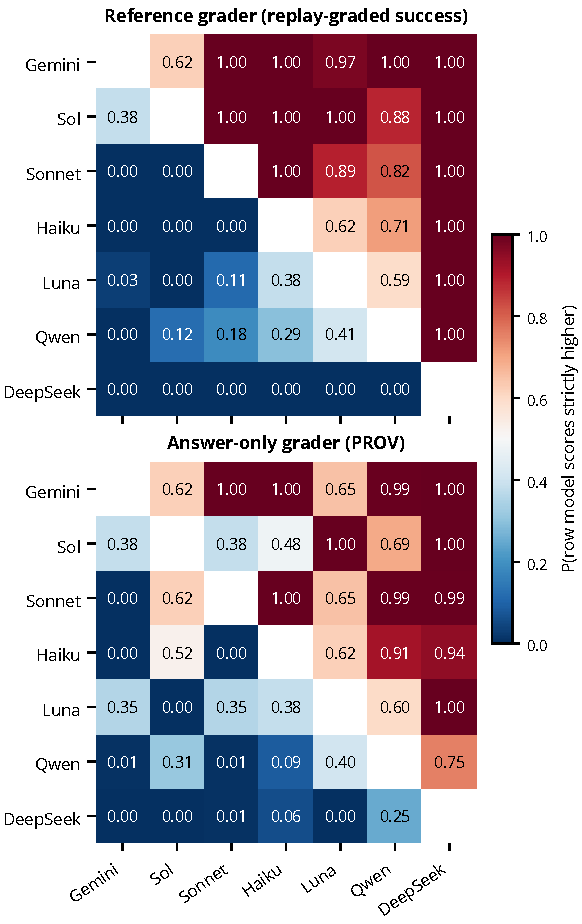
\includegraphics[width=0.72\linewidth]{figures/app_pairwise.pdf}
  \caption{\textbf{v1 pairwise ordering probabilities.} Each cell gives the
  bootstrap probability ($B=20{,}000$, task-cluster) that the row model
  scores strictly higher than the column model, under the reference grader
  (top, replay-graded success) and the answer-only grader (bottom, measured \cfg{Prov}
  score on the same traces). Ties count as not higher, so $P(a>b)+P(b>a)\le1$. Sol is GPT-6.1-sol and Luna is GPT-6-luna.}
  \label{fig:pairwise}
\end{figure}

\subsection{Three populations of uncertainty}
The paper reports three kinds of interval, each over a different population:
\begin{itemize}
\item Wilson intervals in Appendix~\ref{app:dgp-mc} describe the sampling
distribution of \emph{simulated} datasets under deterministic policies, with
no LLM involved.
\item Task-cluster bootstrap intervals describe uncertainty over the task
distribution for a \emph{fixed model panel} with the observed agent outputs.
\item Neither covers run-to-run stochasticity of live model calls beyond what
the repeats contain.
\end{itemize}
These intervals must not be combined.

% ======================================================================
\section{Detailed Results}
\label{app:results}
\begin{table}[t]
\centering
\caption{Paired change vs.\ the reference pipeline (pp; 95\% task-cluster bootstrap CI,
$B=20{,}000$). Regrade rows change only credit on identical traces; fresh rows change replay-graded success (v1) or joint
valid success (v2), which are different constructs. Fault $p$-values: Holm-adjusted task-level sign-flip tests
(v1: 0.023, 0.006, 0.006; v2: all $\ge 0.56$ raw, 1.0 adjusted).
\emph{Visible}: share of faulted runs in which a faulty observation reached the agent.
\emph{LOMO}: range when each model is left out.}
\label{tab:main}
\small
\begin{tabular}{llrrrr}
\toprule
Fault & Comparison & $\Delta$ & 95\% CI & Visible & LOMO range\\
\midrule
\multicolumn{6}{l}{\textit{Original protocol: agent-authored confirm script; 20 tasks, 7 models, 3 repeats}}\\
\cfg{Prov} & same-trace regrade & $+4.5$ & $[+1.9, +7.9]$ & --- & $[+2.8, +5.3]$\\
\cfg{Leak} & fresh runs & $-3.6$ & $[-5.5, -1.4]$ & 89\% & $[-4.4, -1.4]$\\
\cfg{Silent} & fresh runs & $-5.0$ & $[-7.4, -2.6]$ & 28\% & $[-5.8, -3.6]$\\
\cfg{Stale} & fresh runs & $-5.0$ & $[-7.4, -2.6]$ & 44\% & $[-6.1, -2.2]$\\
\midrule
\multicolumn{6}{l}{\textit{Trusted one-shot confirmation: 40 new tasks, 4 models, 1 repeat}}\\
\cfg{Prov\_grade} & same-trace regrade & $+3.1$ & $[+0.6, +5.6]$ & --- & $[+0.0, +4.2]$\\
\cfg{Sep\_read} & fresh runs & $+0.6$ & $[-2.5, +4.4]$ & 88\% & $[+0.0, +1.7]$\\
\cfg{Int\_mask} & fresh runs & $-1.9$ & $[-5.6, +2.5]$ & 15\% & $[-3.3, -0.8]$\\
\cfg{Fresh\_cache} & fresh runs & $-1.2$ & $[-4.4, +1.9]$ & 19\% & $[-2.5, +0.8]$\\
\bottomrule
\end{tabular}
\end{table}

\begin{table}[t]
  \centering
  \small
  \begin{tabularx}{\linewidth}{@{}l>{\raggedleft\arraybackslash}X rrrrrr@{}}
    \toprule
    Config & Measured & Valid & Infl. & FD$_\text{null}$ & Withheld & No sub. & Repro. \\
    \midrule
    \cfg{Ref} & 86.7 & 86.7 [74.3, 95.7] & +0.0 & 13.8 & 11.0 & 1.7 & 87.1 \\
    \cfg{Leak} & 83.1 & 83.1 [71.2, 92.6] & +0.0 & 13.3 & 11.9 & 2.9 & 87.9 \\
    \cfg{Silent} & 81.9 & 81.7 [68.6, 91.7] & +0.2 & 14.3 & 11.9 & 3.1 & 85.7 \\
    \cfg{Stale} & 81.7 & 81.7 [68.6, 91.0] & +0.0 & 13.8 & 9.8 & 5.2 & 79.3 \\
    \cfg{Prov} & 91.2 & 86.7 [75.0, 95.7] & +4.5 & 13.8 & 11.0 & 1.7 & 87.1 \\
    \bottomrule
  \end{tabularx}
  \caption{Pooled results by pipeline configuration (\%, all models). Measured: the configuration's own grader. Valid: replay-graded success (correct and supported by reference replay of the agent's script; not independent evidential validity), with 95\% task-clustered bootstrap CI. Infl.: measured minus valid. FD$_\text{null}$: false discoveries on null tasks. No sub.: no usable submission. Repro.: task cells where all three repeats agree. \cfg{Prov} reuses \cfg{Ref} traces with a grader that skips the provenance check.}
  \label{tab:configs}
\end{table}

\begin{table}[t]
  \centering
  \small
  \begin{tabular}{@{}lrrrrrr@{}}
    \toprule
    Model & \cfg{Ref} & \cfg{Leak} & \cfg{Silent} & \cfg{Stale} & \cfg{Prov} (meas.) & \$/run \\
    \midrule
    Gemini 4 Argon & 95.0 & 93.3 & 91.7 & 95.0 & 95.0 & 0.054 \\
    GPT-6.1-sol & 91.7 & 93.3 & 91.7 & 91.7 & 91.7 & 0.022 \\
    Sonnet 5.5 & 90.0 & 90.0 & 86.7 & 90.0 & 95.0 & 0.035 \\
    Haiku 5.5 & 88.3 & 90.0 & 86.7 & 90.0 & 93.3 & 0.003 \\
    GPT-6-luna & 86.7 & 83.3 & 80.0 & 83.3 & 90.0 & 0.002 \\
    Qwen3.8-flash & 85.0 & 78.3 & 71.7 & 63.3 & 88.3 & 0.012 \\
    DeepSeek-V4.1-flash & 70.0 & 53.3 & 63.3 & 58.3 & 85.0 & 0.016 \\
    \bottomrule
  \end{tabular}
  \caption{Replay-graded success (\%) by model and configuration (v1); \cfg{Prov} column shows the measured score of the same \cfg{Ref} traces under a grader without the provenance check. Mean API cost per \cfg{Ref} run in USD.}
  \label{tab:models}
\end{table}

\begin{table}[h]
\centering
\caption{\textbf{v2 joint valid success (\%) by model and condition} (unit: run; 40 tasks per cell, one
repeat). \emph{Prov.}: answer-only credit on the same \cfg{Ref} traces. \emph{Protocol}: share of all 160
runs of the model with a valid protocol. \emph{Calls}: mean model calls per run. \emph{\$/run}: mean
recorded OpenRouter cost.}
\label{tab:v2models}
\small
\begin{tabular}{lrrrrrrrr}
\toprule
Model & \cfg{Ref} & \cfg{Sep\_read} & \cfg{Int\_mask} & \cfg{Fresh\_cache} & Prov. & Protocol & Calls & \$/run\\
\midrule
GPT-6.1-sol & 92.5 & 92.5 & 92.5 & 92.5 & 92.5 & 100.0 & 4.0 & 0.0122\\
Haiku 5.5 & 82.5 & 80.0 & 77.5 & 85.0 & 95.0 & 85.6 & 3.8 & 0.0016\\
GPT-6-luna & 92.5 & 95.0 & 95.0 & 92.5 & 92.5 & 100.0 & 5.5 & 0.0008\\
DeepSeek-V4.1-fl. & 92.5 & 95.0 & 87.5 & 85.0 & 92.5 & 96.9 & 12.3 & 0.0037\\
\bottomrule
\end{tabular}
\end{table}


\textbf{Abstention and termination.} Of 1,680 v1 runs, 54 ended at the step
limit, 7 of them in \cfg{Ref}. In v2, no run used \texttt{abstain}. Five of
640 runs ended without a submission, all DeepSeek and all under
\cfg{Int\_mask} (2) or \cfg{Fresh\_cache} (3); none occurred in \cfg{Ref} or
\cfg{Sep\_read}. Mean model calls per v2 run were 6.1 (\cfg{Ref}), 6.0
(\cfg{Sep\_read}), 6.5 (\cfg{Int\_mask}), and 7.0 (\cfg{Fresh\_cache}). Mean
failing executions per run were 0.47 under \cfg{Int\_mask} and 0.11 in
\cfg{Ref}.

% ======================================================================
\section{Reproducibility and Implementation}
\label{app:repro}

\textbf{Repository layout} (code, frozen records, and analyses; prepared for release):
\begin{itemize}
\item \texttt{scieval/}: the v1 harness, comprising tasks, pipeline and
faults, agent loop, grader, runner, replay, probes, and the original analyses
and figures.
\item \texttt{research\_v2/}: the oracle, v2 harness, agent loop and runner,
validator, fault contracts, instrumentation (\texttt{audit\_runner.py},
\texttt{audit\_existing.py}), analyses (\texttt{decompose\_v1.py},
\texttt{analysis\_v1.py}, \texttt{analysis\_v2.py}, \texttt{stats.py},
\texttt{dgp\_validation.py}), table and figure generators, and tests.
\item \texttt{research\_v2/frozen/}: the inputs, comprising
\texttt{runs\_v1\_main.tar.gz} (all 1,680 v1 records with full events and
messages), \texttt{suites.tar.gz} (both task suites),
\texttt{confirm\_audit.jsonl}, \texttt{runs\_v2/}, the v2 task manifest with
SHA-256 hashes of every split, and OpenRouter model and endpoint metadata
retrieved 2026-10-25.
\end{itemize}

\textbf{Record counts.} \texttt{runs\_v2/v2main} holds 800 records: the 640
model runs and 160 reference-agent runs (40 tasks $\times$ 4 conditions,
\$0). \texttt{runs\_v2/smoke2} holds 26 smoke-test records (\$0.12). They
used 2 tasks, are excluded from all analyses, and include the Qwen3.8-flash
smoke run that led us to drop that model for latency. Each v2 record stores
settings, oracle version, package versions, the submission, validation, fault
manifestation, issued evidence records, usage, per-call metadata, events, and
messages. Per-call metadata comprises request id, returned model, provider,
cost, latency, and timestamp. Runs that hit an API error were not saved and
were retried. The returned provider equalled the pin in every call.

\textbf{Inference settings (v2).} The four models are:
\begin{itemize}
\item \texttt{openai/gpt-6.1-sol} (snapshot 2026-09-29), pinned to OpenAI;
\item \texttt{anthropic/claude-haiku-5.5} (2026-10-07), pinned to Anthropic;
\item \texttt{openai/gpt-6-luna} (2026-09-22), pinned to OpenAI;
\item \texttt{deepseek/deepseek-v4.1-flash} (2026-09-10), pinned to DeepInfra
fp8.
\end{itemize}
All requests used \texttt{allow\_fallbacks=false} and
\texttt{require\_parameters=true}, reasoning effort \texttt{low},
\texttt{max\_tokens=4096}, at most 20 model calls with a budget notice at call
17, seed $10{,}000+\text{repeat}$ where listed as supported, and temperature
0 only for DeepSeek, whose endpoint lists it. Costs were GPT-6.1-sol \$1.96,
DeepSeek \$0.56, Haiku \$0.26, and GPT-6-luna \$0.13. v1 used router-default
endpoints and sampling, which cannot be reconstructed.

\textbf{Environment.} Python 3.12.12, numpy 2.5.4, scipy 1.18.1, pandas
3.1.0, statsmodels 0.15.0, and pytest 9.1.1 on macOS with
\texttt{sandbox-exec}.

\textbf{Offline regeneration.} \texttt{bash research\_v2/reproduce\_offline.sh}
needs no API key or network. It restores the frozen archives into the cache
if needed, runs the 15 tests, regenerates the Monte Carlo study, the v1
decomposition and analysis, the v2 analysis, all figures and tables, and the
pipeline figure, and compiles this PDF. Re-executing the v1 confirmation
scripts is optional (\texttt{REAUDIT=1}; macOS only); otherwise the frozen
\texttt{confirm\_audit.jsonl} is used. The analysis is deterministic given
the frozen records and the bootstrap seed. Live model calls are not
reproducible bit-for-bit even with pinned endpoints and seeds, which is why
records are frozen.

\begin{center}\footnotesize
\begin{tabular}{p{4.2cm}p{5.0cm}p{5.0cm}}
\toprule
Artifact & Generator & Inputs\\
\midrule
Figure~\ref{fig:pipeline} & \texttt{paper/figures/src/pipeline.tex} & ---\\
Figure~\ref{fig:effects} & \texttt{research\_v2/figures\_v2.py} & \texttt{results/v1,v2/summary\_*.json}, \texttt{prov\_newly\_credited.csv}\\
Tables~\ref{tab:main}, \ref{tab:dgp} & \texttt{tables.py}, \texttt{appendix\_tables.py} & summaries; \texttt{dgp\_validation\_summary.json}\\
Tables~\ref{tab:power}--\ref{tab:lomo}, \ref{tab:v2models}; Figs.~\ref{fig:tec}, \ref{fig:manifest}, \ref{fig:pairwise} & \texttt{research\_v2/appendix\_tables.py} & \texttt{v1\_per\_run.csv}, \texttt{v2\_per\_run.csv}, \texttt{confirm\_audit.jsonl}, frozen v1 records\\
Tables~\ref{tab:configs}, \ref{tab:models} & \texttt{scieval/analyze.py} & frozen v1 records\\
All v1 statistics & \texttt{decompose\_v1.py}, \texttt{analysis\_v1.py} & frozen v1 records, \texttt{confirm\_audit.jsonl}, \texttt{results/main/fixed\_replay.json}\\
All v2 statistics & \texttt{analysis\_v2.py} & \texttt{frozen/runs\_v2/v2main}\\
\bottomrule
\end{tabular}
\end{center}

% ======================================================================
\section{Construct and External Validity}
\label{app:validity}

\textbf{Truth versus evidence.} Even with a correctly specified analysis, a
finite confirmation sample supports a false claim with probability about
$\alpha$ under the null, and the reference agent fails to confirm a true effect in 1--27\% of
pairs across our effect bins, through selection or power (Table~\ref{tab:power}). \fld{truth} and
\fld{evid} therefore diverge by design, and a benchmark must decide which
it is measuring.

\textbf{What counts as correct.} Five acts must be kept apart:
\begin{itemize}
\item identifying the true exposure;
\item following the decision rule;
\item reporting a confirmed discovery;
\item withholding an unsupported claim;
\item giving affirmative evidence of no effect.
\end{itemize}
Our protocol scores the first through \fld{truth} and the second and third
through \fld{evid}/\fld{cons}. It treats the fourth (ncd) as
truth-correct on null tasks because no false claim is made. It never scores
the fifth, which would need an equivalence test.

\textbf{A frozen oracle.} Fixing OLS with site indicators is legitimate here
because it is the correctly specified model for the generator. In practice,
the choice of analysis is part of the science. A trusted protocol for real
data would pre-register an analysis family (model, covariates, estimand, and
error control) and execute it server-side. It would not fix one formula for
all tasks.

\textbf{Generalization.} All findings are measured on one linear-inference
family. The four framings change names, not statistics. Three findings
concern infrastructure and plausibly carry over to any benchmark where
agents write confirmatory code or where credit can be earned without
evidence: label-based provenance checks measure format, unrestricted
confirmation does not bound the number of tests, and answer-only grading
rewards untested negative decisions. We have not tested them elsewhere. The
magnitudes are specific to this family, these models, and these fault
implementations.

\textbf{Protocol versus capability.} v2 delegates the confirmatory
computation to the harness on purpose, because the object of study is
measurement validity. A high v2 score certifies hypothesis selection and
decision discipline. It does not certify the ability to design or implement
an analysis, which a separate, harder benchmark must measure.

\textbf{Scope.} The panels are fixed: 7 models in v1 and 4 in v2. v1 used
router-default inference and 3 repeats, v2 one repeat and pinned low-effort
reasoning. Each redesigned fault has one implementation, and the two studies
differ in many ways at once (\S\ref{app:faults-compare}).

\textbf{Recommendations.} Each follows from a result above:
\begin{itemize}
\item execute confirmatory analyses in the harness, with the hypothesis
locked before the result is visible (\S\ref{sec:multitest});
\item bind decisions to evidence by identifier and type the decision field
(\S\ref{sec:prov}, \S\ref{app:labels});
\item report \fld{truth}, \fld{evid}, \fld{cons}, \fld{proto},
and abstention separately, and never credit a negative decision without
evidence on null-heavy benchmarks (\S\ref{sec:prov});
\item benchmark false discoveries against a trusted agent on the same
datasets, and count datasets rather than runs (\S\ref{sec:diverge});
\item report trigger, visibility, and use with every injected fault
(\S\ref{sec:env});
\item deny reads outside the agent's workspace (\S\ref{app:faults-v1}).
\end{itemize}

\textbf{Original conformance probes (v1).} The v1 study also scored each
configuration with 15 unweighted conformance probes in
\texttt{scieval/probes.py}: 6 integrity, 4 freshness, 3 separation, and 2
provenance. Each faulted configuration fails only its own rule's probes, so
pass rates are \cfg{Prov} 0.87, \cfg{Leak} 0.80, \cfg{Stale} 0.73, and
\cfg{Silent} 0.67. The highest-scoring configuration was the only one that
inflated credit. This shows that invariant coverage and the consequence of
violating an invariant are different quantities, not that conformance
testing is uninformative.
